\chapter{Softwarearchitektur}
Softwarearchitektur beschäftigt sich mit dem Erstellen des Fundamentes eines Softwareprojektes \cite[S. 9]{softarch}. Der Fokus liegt daher nicht auf Implementationsdetails sondern auf Schnittstellen, welche das System und die Zusammenarbeit der Teilkomponenten beschreiben \cite[S. 8]{basiswissen}. Ziel der Softwarearchitektur ist es, durch Abstraktion der Details einen Überblick über die zu implementierenden Komponenten zu gewinnnen, welcher es ermöglicht, frühe Entscheidungen über die Probleme und Angemessenheit des Systems zu erlangen und somit Risiken, Fehler- und Änderungskosten zu vermeiden oder zu verringern \cite[S. 10]{softarch}.

\section{Architektursichten}
Der Detailgrad der Schnittstellen hängt wesentlich von der Größe des Projektes ab \cite[S. 7-12]{basiswissen}. Um die Komplexität und Abstraktion zu beherrschen, können Architektursichten verwendet werden, welche einen Überblick über Teilbereiche des Systems ermöglichen \cite{ISO_ARCH}. Ein Beispiel dafür ist Kruchtens 4+1 Sichtenmodell \cite{kruch}, welches folgende Sichten beschreibt:

\begin{itemize}
  \item Logical View: Logische Sicht auf das System, welches die Klassen und deren Beziehungen untereinander darstellt
  \item Process View: Beschäftigt sich mit nicht funktionalen Anforderungen wie Performance und Fehlertolleranz und deren Implementierung
  \item Development View: Beschreibt die Aufteilung des Systems in Module und Bibliotheken
  \item Physical View: Regelt und beschreibt die Verteilung der Komponenten auf physische Systeme
  \item Scenarios: Usecases, welche die Nutzung des Systems beschreiben
\end{itemize}

Kruchten verwendet eigene Diagramme für jede Sicht, die an UML angelehnt aber zum Teil verschieden sind, etablierte sich UML doch erst zwei Jahre später nach der Veröffentlichung seines Modelles \cite{glasklar}[S. 5].

Es gibt noch viele andere Sichtenmodelle wie das Zachman Framework \cite[S. 282]{zachman}, welches eine Aufteilung in Kontext-, Geschäfts, System, Technologie, Integrations und Laufzeitsicht vornimmt. Die Gemeinsamkeit aller Sichtenmodelle ist jedoch der Versuch, durch unterschiedliche Sichtweisen einen besseren Überblick über das Zielsystem zu erlangen.



\section{Architekturprozess Lifecycle}
Zeitlich ordnet sich die Architekturphase zwischen dem Ermitteln der Anforderungen und der tatsächlichen Implementation ein. Da die Erstellung von Software heutzutage mehr ein agiler und inkrementeller Prozess ist, wird auch die Erstellung und die Mitwirkung der Softwarearchitektur in diese sich wiederholenden Prozesse mit einbezogen. \cite[S. 7]{basiswissen}

Der Architekturzyklus lässt sich mit dem in Abbildung \ref{fig:cycle} beschriebenen Aktivitätsdiagramm darstellen und unterteilt sich in folgende Unterbereiche \cite[Umschlag]{softarch}:

\begin{itemize}
  \item \glqq Erstellen der Systemvision\grqq
  \item \glqq Verstehen der Anforderungen\grqq
  \item \glqq Entwerfen der Architektur\grqq
  \item \glqq Umsetzen der Architektur\grqq
  \item \glqq Kommunizieren der Architektur\grqq
\end{itemize}


\begin{figure}[H]
    \centering
    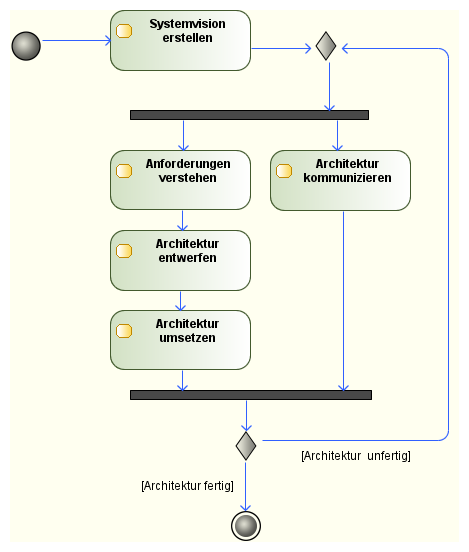
\includegraphics[scale=0.8]{img/archcycle.png}
    \caption{Der Architekturprozess modelliert als Aktivitätsdiagramm \cite[Umschlag]{softarch}}
    \label{fig:cycle}
\end{figure}

Der Fokus der Arbeit liegt wegen der fehlenden Implementierung hauptsächlich auf den ersten drei Teilen, der Erstellung der Systemvision, Verstehen der Anforderungen und dem Entwerfen der Architektur.

\section{Was macht eine gute Softwarearchitektur aus}
Die Frage, was eine gute Softwarearchitektur ausmacht, wird oft sehr breit und ungenau beantwortet: Eine gute Architektur erfülle die \glqq Verhaltens-, Qualitäts- und Lebenszyklusanforderungen\grqq \ \cite[S. 12]{basiswissen} eine Systems, ermögliche es Risiken frühzeitig zu erkennen und die inhärente Komplexität eines Systems und dessen Quellcodes zu beherrschen \cite[S. 7-8]{softarch}.

Alle diese Kriterien lassen sich jedoch schwierig oder gar nicht messen. Manche Werte sind zwar messbar, aber lassen keine eindeutigen Entscheidungen ableiten: zB. können Kopplung und Kohäsion eines Systemes gemssen werden, jedoch kann nicht eindeutig festgelegt werden, ab welchem Wert die Kopplung zu hoch oder die Kohäsion zu niedrig ist.

Dieter Masek kommt zu folgendem Schluss: \glqq Die Frage ob eine gegebene Architektur gut oder schlecht ist, lässt sich nicht direkt beantworten. Gut oder schlecht sind absolute Bewertungen, die für Architekturen sowieso nicht möglich sind. Eine Architektur lässt sich nur in einem festgelegten Kontext beurteilen d.h.: Wie gut löst eine Architektur ein vorgegebenes Problem? Selbst diese eingeschränkte Frage lässt sich nicht mit gut oder schlecht beantworten! \grqq \ \cite[S. 19]{review}

Trotz all dieser Probleme lassen sich dennoch Werte messen und überprüfen \cite[S. 19]{review}, welche in Verbindung mit unzureichenden Architektureintscheidungen gebracht werden können. Dies erlaubt folgenden Schluss: Die Ausgangsfrage, was eine gute Softwarearchitektur ausmacht, führt zu keiner Erkenntnis und ist damit mehr oder minder nutzlos: Es kommt nicht darauf an, ob eine Architektur gut ist, sondern ob eine Architektur die an sie gestellten Anforderungen erfüllt.

Viele dieser Anforderungen stehen im Gegensatz zueinander: zB. erfordert eine hohe Performance eine niedrigere Abstraktionsebene, was jedoch die Wartung des Codes erschwert. Die Findung einer angemessene Softwarearchitektur beschäftigt sich somit mehr mit der Abwägung von Vor- und Nachteilen, welche aus den jeweiligen Entwurfsmustern und Technologien ableitbar sind.

Um diese Entscheidungen abwägen zu können, ist wichtig, die expliziten Anforderungen an das System zu kennen \cite[S. 19]{review}. Eine möglichst vollständige Anforderungsanalyse ist somit die Ausgangsbasis für eine angemessene Softwarearchitektur. Dies kann jedoch vor allem am Anfang der Anforderungsanalyse schwierig sein, da die KundInnen noch keine genaue Vorstellung vom zu entwickelnden System haben \cite[S. 80]{reqman}.

Eine Möglichkeit zur Überprüfung von bestehenden und noch nicht beachteteten Anforderungen der Architektur stellt die Durchführung eines szenariobasierten Architekturreviews wie ATAM oder CBAM dar.


\section{Architekturbewertungsmethoden}
Architekturbewertungsmethoden werden dazu verwendet, die Angemessenheit einer Architektur zu überprüfen. Die Meisten ihrer Art basieren auf der Erstellung von Szenarien, da das Kosten-Nutzen Verhältnis dieser Herangehensweise sehr gut ist \cite[S. 185]{basiswissen}.

Es gibt mehrere verschiedene Bewertungsmethoden wie CBAM, ALMA und ARID, welche zum Großteil Abwandlungen von ATAM darstellen. ATAM wiederum ist eine Weiterentwicklung von SAAM. \cite[S. 60-76]{review}

Da Kosteneffektivität, Änderungs- und Wachstumsszenarien die Basis für Entscheidungen des erstellten Architekturprozesses darstellen, wird näher auf ATAM (Änderungs- und Wachstumsszenarien) und CBAM (Kostenszenarien) eingegangen.

\subsection{ATAM}
ATAM, kurz für Architecture Trade-off Analysis Method, beschäftigt sich mit den nicht funktionalen Anforderungen wie Performance oder Verfügbarkeit. Sie lässt sich in folgende Phasen einteilen \cite[S. 185]{basiswissen}:

\begin{itemize}
  \item Vorbereitungsphase
  \item Architekturzentrierte Bewertung
  \item StakeholderInnenzentrierte Bewertung
  \item Nachbearbeitungsphase
\end{itemize}

Einer initialen Vorbereitungsphase, in welchem das Team und der Zeitplan erstellt wird, folgt ein Treffen mit den StakeholderInnen des/der AuftraggeberIn, in der die Geschäftsziele und Architektur vorgestellt werden. In diesem Treffen werden die nicht funktionalen Anforderungen anhand eines Utilitytrees erarbeitet, priorisiert und bewertet. Sind wichtige architekturrelevante Anforderungen noch nicht bekannt, können diese nun mit den StakeholderInnen erarbeit werden. \cite[S. 184-199]{basiswissen}

Auf Basis des Utilitytrees und dessen nicht funktionale Anforderungen werden dann in den darauf folgenden Bewertungsphasen folgende Szenarientypen überprüft \cite[S. 62-67]{review}\cite[S. 188]{basiswissen}:

\begin{itemize}
  \item Usecases
  \item Wachstumsszenarien
  \item Explorative Änderungsszenarien
\end{itemize}

Die Usecases beschreiben die Standardanwendungsfälle der NutzerInnen, welche durch das System umgesetzt werden sollen. Auch sie werden priorisiert. Danach führen die ArchtektInnen pro Usecase eine Analyse der im Utilitytree beschriebenen nicht funktionalen Anforderungen durch. Je nachdem, wie viel Zeit für die Analyse aufgewendet werden soll, werden zusätzlich zu den als hoch priorisierten Usecases und nicht funktionalen Anforderungen auch weitere, niedriger Priorisierte überprüft. \cite[S. 192]{basiswissen}

Sind die Bewertungsphasen abgeschlossen können die Ergebnisse analysiert und dokumentiert werden. Dies dient nicht nur als Dokumentation der geplanten Verbesserungen für die Architekturplanung, sondern hilft auch in zukünftigen ATAM Analysen die Entscheidungen früherer Analysen nachzuvollziehen. \cite[S. 189]{basiswissen}


\subsection{CBAM}